% !TeX root = ../../main.tex

% \subsection{Simplicial Complexes}\label{sec:complexes}

A \textbf{simplicial complex} $K$ is a collection of subsets, called \textbf{simplices}, of a vertex set $V$ such that for all $\sigma\in K$ and $\tau\subset\sigma$ it must follow that $\tau\in K$.
The \textbf{dimension} of a simplex $\sigma\in K$ is defined as $\dim(\sigma) := |\sigma|-1$ where $|\cdot|$ denotes set cardinality.
The dimension of a simplicial complex $K$ is the maximum dimension of any simplex in $K$.
That is, a graph is a 1-dimensional simplicial complex in which vertices and edges are 0 and 1-dimensional simplices, respectively.

% \figblock{%
% \begin{figure}[htbp]
% \centering
%     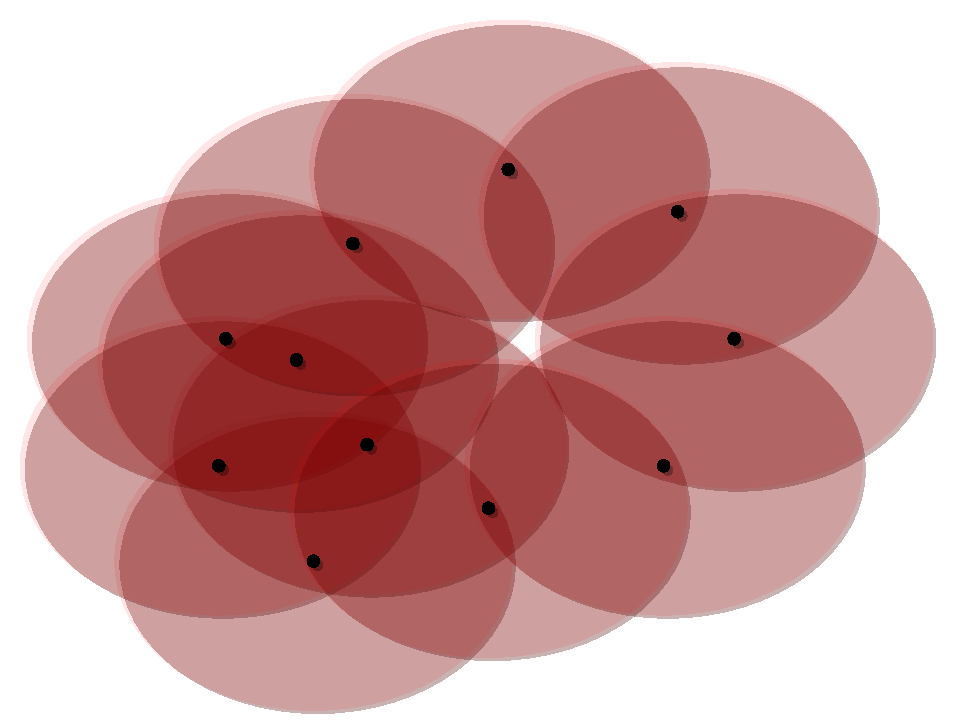
\includegraphics[scale=0.33]{figures/holes_cover.pdf}
%     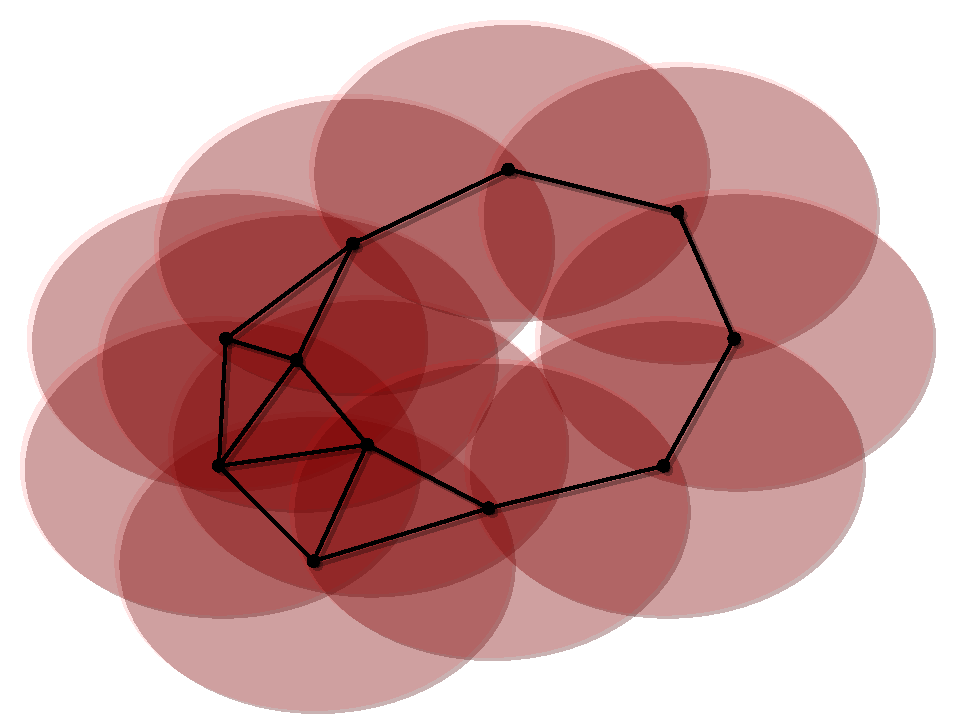
\includegraphics[scale=0.33]{figures/holes_edges.pdf}
%     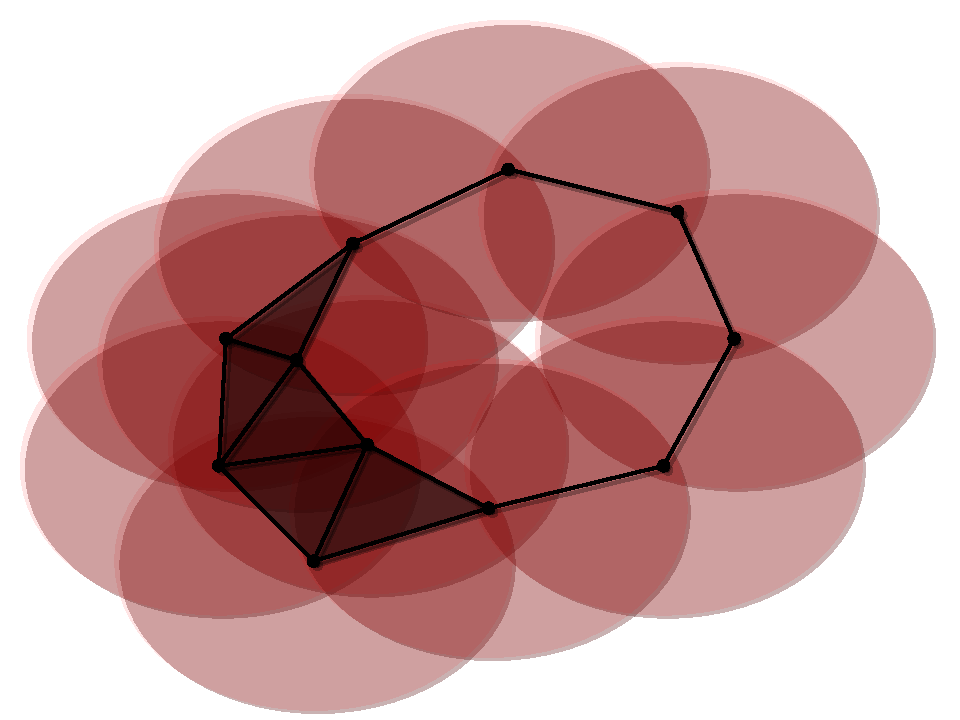
\includegraphics[scale=0.33]{figures/holes_complex.pdf}
%      \caption{(Left) The coverage regions of a collection of points $P$ at some scale $\alpha$.
%             (Middle) The neighborhood graph with edges for each pair of points within pairwise distance $\alpha$.
%             (Right) If we attempt to fill cycles in the graph with triangles identify a cycle that cannot be filled which reflects a gap in coverage}
%      \label{fig:holes}
% \end{figure}}

It is natural to think of a $k$-dimensional simplicial complex as the generalization of an undirected graph consisting of vertices and edges, collections of at most 2 vertices, to collections of sets of at most $k-1$ vertices.
% Just as we have defined a hole in our graph $G$ as a cycle that cannot be filled with triangles, we define a $k$-dimensinal hole in a simplicial complex as a $k$-cycle that cannot be filled with $(k+1)$-simplices.
% In the next section we will formally define $k$-cycles and introduce simplicial homology as a tool for identifying when and which cycles cannot be filled.

\paragraph{Coordinate-free Communication}
% In a coordinate-free sensor network each sensor, represented by a point in $P$, is capable of detecting nodes which are sufficiently ``close.''
% That is, there is some radius of communication $\delta > 0$ such that two nodes $p, q\in P$ such that $\dist(p, q) \leq\delta$ are capable of communication.
% Note that, although sensors can communicate within this distance they are not able to measure the distance itself.

Let $P$ be a finite collection of points in a subspace $D$ of some (unknown) metric space $X$.
In a coordinate-free setting we are only provided with limited information about the connectivity of points in $P$.
We do not know the precise locations of the points, nor the distances between them.
For example, in coordinate-free sensor networks each sensor is represented by a point in $P$ and there is some distance $\e > 0$ that sensors can communicate within, but not able measure.

With this limited capability we can construct an undirected graph $G=(V, E)$ with vertices $V=P$ and edges $E = \{\{p, q\}\subset P\mid \dist(p,q)\leq\delta\}$.
Let $K$ be a simplicial complex with 0-simplices $\{v\}$ for all $p\in P$, 1-simpices $\{u, v\}\subset P$ for each edge in $E$, and 2-simplices $\{u,v,w\}\subset P$ whenever $\{\{\{u,v\},\{v,w\},\{u,w\}\}\subset E$.
This particular simplicial complex is known as the Vietoris-Rips complex.
It is also an example of a clique complex, where the simplices are the complete subgraphs (or cliques) in a given graph.

Formally, the \textbf{(Vietoris-)Rips complex} is defined for a finite set $P$ at scale $\e > 0$ as
\[ \rips^\e(P) = \left\{\sigma \subseteq P\mid \forall p,q\in\sigma,\ \dist(p, q)\leq \e\right\}. \]
For a pair $(P, Q)$ we will write $\rips^\e(P,Q) := (\rips^\e(P), \rips^\e(Q))$ to denote the corresponding pair of rips complexes.

\paragraph{Coverage}
% In order to determine coverage we must at least assert that the coverage domain spanned by the points in $P$ does not contain any holes.
% Assuming the coverage radius of our sensors is equal to their communication radius $\delta$ we may define a hole in coverage as a cycle that cannot be ``filled'' with triangles (see Fig.~\ref{fig:holes}).

% \figblock{%
% \begin{figure}[htbp]
% \centering
%     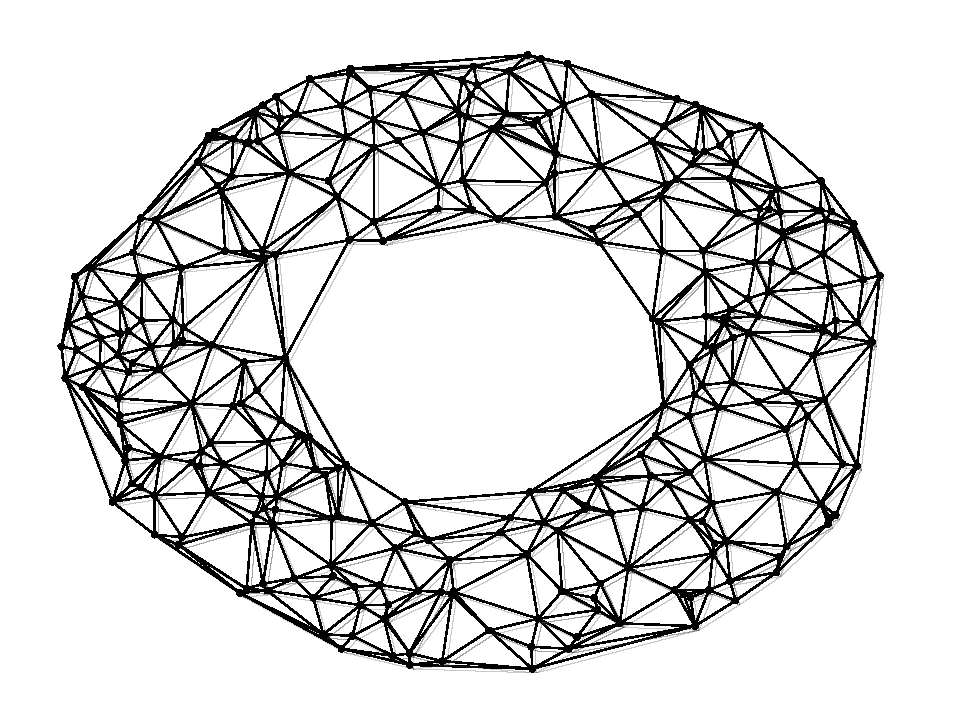
\includegraphics[scale=0.33]{figures/boundary_graph.pdf}
%     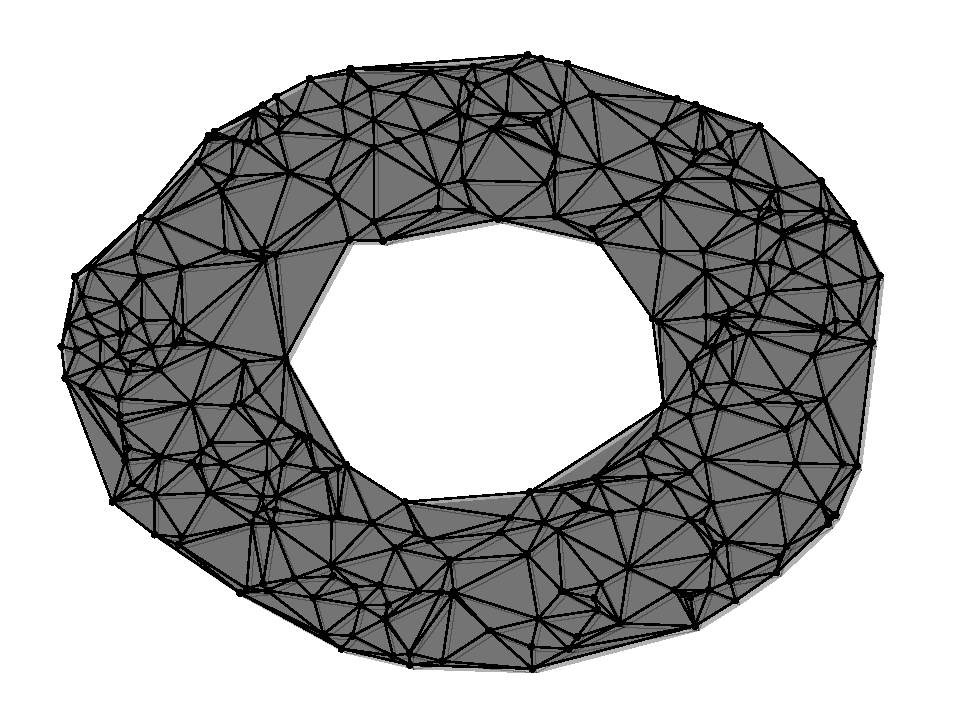
\includegraphics[scale=0.33]{figures/boundary_complex.pdf}
%     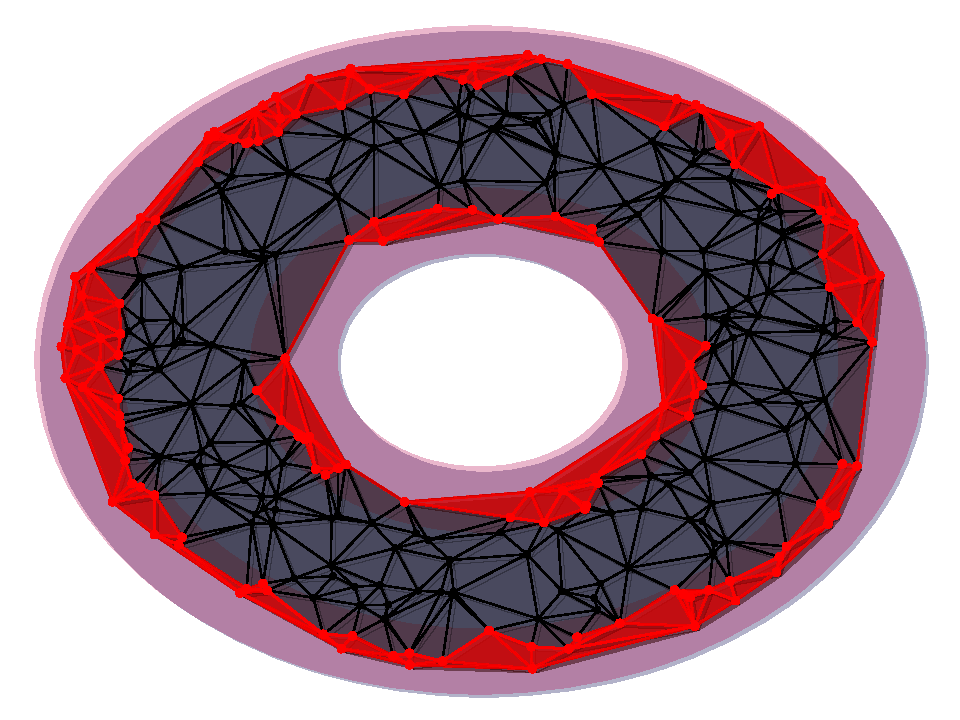
\includegraphics[scale=0.33]{figures/boundary_complex_domain_fence.pdf}
%     % 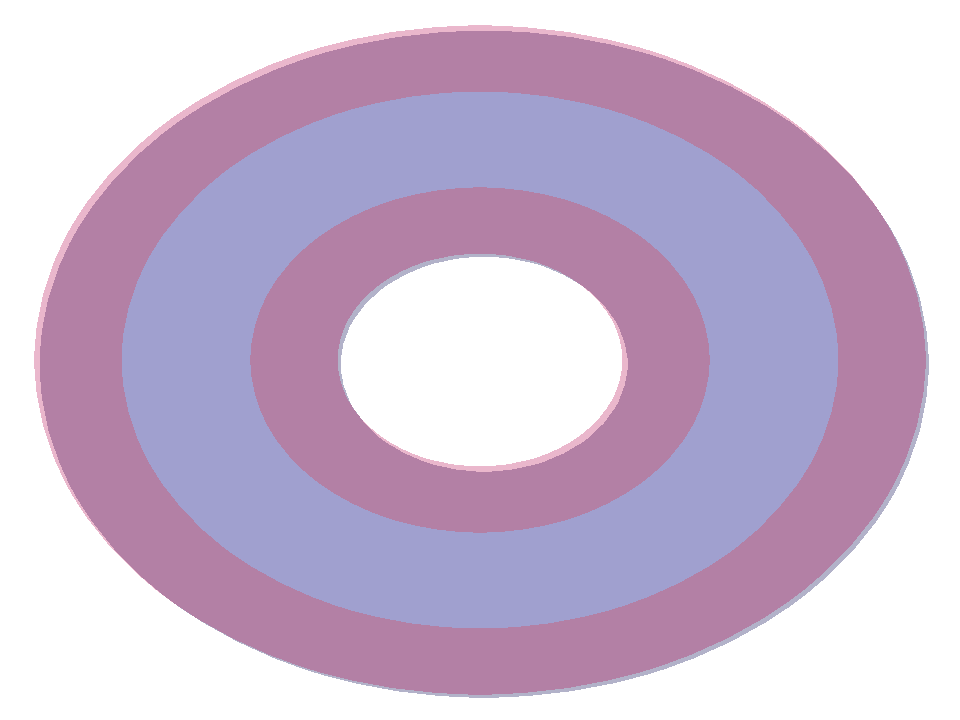
\includegraphics[scale=0.24]{figures/boundary_domain.pdf}
%      \caption{(Left) The neighborhood graph of a sensor network with a large ``hole''.
%             (Middle) A 2-dimensional simplicial complex with no gaps in coverage, but an unfilled cycle.
%             (Right) By allowing nodes to identify the boundary (in red) we can confirm coverage of complex domains.}
%      \label{fig:boundary1}
%  \end{figure}}

If $D\subseteq P^\e$ then we say that the collection of points $P$ covers $D$ at scale $\e$.
In this case, the topology of the domain is reflected in $\rips^\e(P)$.
However, as we will see, this may not give a tight bound on the minimum radius for coverage.
In fact, if the coverage region of of a sensor network at scale $\e$ has no gaps, then the minimum coverage radius required is a constant factor smaller than $\e$.
We will therefore use a sequence of rips complexes in order to approximate a simplicial complex which captures the homotopy type of the cover.
% This point is made clear by an interleaving of the Rips with another simplicial complex known as the \v Cech complex.

The \textbf{\v Cech complex} of a finite collection of points $P$ at scale $\e > 0$ is defined
\[ \cech^\e(P) = \left\{\sigma \subseteq P\mid \bigcap_{p\in \sigma}\ball_\e(p)\neq \emptyset \right\}. \]
The \v Cech and Rips complexes of a finite metric space are closely related by a result that follows from Jung's Theorem~\cite{jung01uber} relating the diameter of a point set $P$ and the radius of the minimum enclosing ball:
\[\cech^{\e/\jungd}(P)\subseteq\rips^\e(P)\subseteq\cech^\e(P)\subseteq\rips^{\jungd\e}(P),\]
where the constant $\jungd = \sqrt{\frac{2d}{d+1}}$ (see~\cite{buchet15efficient}).
Throughout we will take the lower bound $\jungd = 2$ for more general spaces.

The \v Cech complex is a special case of a more general construction known as the \textbf{nerve} $\N(\cU)$ of a collection of sets $\cU = \{U_i\}_{i\in I}$, where $I$ is any indexing set.
The nerve of $\cU$ is defined as the simplicial complex with vertex set $I$ such that $\sigma\subseteq I$ is a simplex if and only if
\[
  \bigcap_{i\in \sigma} U_i\neq \emptyset.
\]
The collection $\cU$ is a \textbf{good cover} if for each $\sigma\subset I$ the set $\bigcap_{i\in\sigma} U_i$ is contractible or empty.
The \textbf{Nerve Theorem} states that if $\cU$ is a good cover then its nerve $\N(\cU)$ is homotopy equivalent to $\bigcup_{i\in I} U_i$.

That is, for a set of points $P\subset D$ such that $\cU = \{\ball^\e(p)\mid p\in P\}$ is a good cover the nerve $\N(\cU)$ is homotopy equivalent to $P^\e = \bigcup_{p\in P} \ball_\e(p)$.
Noting that the open balls $\ball^\e_D(p)$ are either empty or contractible when $\varrho_D > \e$ then $\cU$ is a good cover in this case, and the inclusion $\cech^\e(P)\hookrightarrow P^\e$ is a homotopy equivalence.
There is still a question of whether this homotopy equivalence induces a homotopy equivalence on pairs $\cech^\e(P,Q)$ and $(P^\e, Q^\e)$ in general, which would require the restriction of the homotopy to $\cech^\e(Q)$ to fall within $Q^\e$, and the restriction of its inverse to $Q^\e$ to fall within $\cech^\e(Q)$.
Proof of this equivalence is beyond the scope of this paper, however we do discuss the persistent case in Appendix~\ref{apx:nerves}.
